%\PassOptionsToPackage{table}{xcolor}
% \documentclass[smaller, dvipsnames,handout,
% hyperref={colorlinks=true,urlcolor=magenta,citecolor=cyan,linkcolor=orange}]{beamer}
\def\bmode{0} % Mode 0 for presentation, mode 1 for a handout with notes, mode 2 fo% r handout without notes
\if 0\bmode
\documentclass[usenames,dvipsnames,smaller]{beamer}
\else \if 1\bmode
\immediate\write18{pdflatex -jobname=\jobname-Handout-Notes\space\jobname}
\documentclass[usenames,dvipsnames,smaller,handout]{beamer}
\usepackage{handoutWithNotes}
\pgfpagesuselayout{2 on 1 with notes}[letterpaper, landscape, border shrink=4mm]
\else \if 2\bmode
\immediate\write18{pdflatex -jobname=\jobname-Handout\space\jobname}
\documentclass[usenames,dvipsnames,smaller,handout]{beamer}
\fi
\fi
\fi



% \documentclass[smaller,handout
% ]{beamer}
%\usepackage{etex}
%\newcommand{\num}{6{} }

% \usetheme[
%   outer/progressbar=foot,
%   outer/numbering=counter,
%  block=fill
% ]{metropolis}

%\useoutertheme{metropolis}

\usetheme{Madrid}
\useoutertheme[subsection=false]{miniframes} % Alternatively: miniframes, infolines, split
\useinnertheme{circles}
\usecolortheme{seahorse}

\usepackage[backend=biber,style=authoryear,maxcitenames=2,maxbibnames=99,safeinputenc,url=false,
eprint=false]{biblatex}
\addbibresource{bib/references.bib}
\AtEveryCitekey{\iffootnote{{\tiny}\tiny}{\tiny}}

%\usepackage{pgfpages}
%\setbeameroption{hide notes} % Only slides
%\setbeameroption{show only notes} % Only notes
%\setbeameroption{hide notes} % Only notes
%\setbeameroption{show notes on second screen=right} % Both

% \usepackage[sfdefault]{Fira Sans}

% \setsansfont[BoldFont={Fira Sans}]{Fira Sans Light}
% \setmonofont{Fira Mono}

%\usepackage{fira}
%\setsansfont{Fira}
%\setmonofont{Fira Mono}
% To give a presentation with the Skim reader (http://skim-app.sourceforge.net) on OSX so
% that you see the notes on your laptop and the slides on the projector, do the following:
% 
% 1. Generate just the presentation (hide notes) and save to slides.pdf
% 2. Generate onlt the notes (show only nodes) and save to notes.pdf
% 3. With Skim open both slides.pdf and notes.pdf
% 4. Click on slides.pdf to bring it to front.
% 5. In Skim, under "View -> Presentation Option -> Synhcronized Noted Document"
%    select notes.pdf.
% 6. Now as you move around in slides.pdf the notes.pdf file will follow you.
% 7. Arrange windows so that notes.pdf is in full screen mode on your laptop
%    and slides.pdf is in presentation mode on the projector.

% Give a slight yellow tint to the notes page
%\setbeamertemplate{note page}{\pagecolor{yellow!5}\insertnote}\usepackage{palatino}


%\usetheme{metropolis}
%\usecolortheme{beaver}
%\usepackage{xcolor}
\definecolor{darkcandyapplered}{HTML}{A40000}
\definecolor{lightcandyapplered}{HTML}{e74c3c}

%\setbeamercolor{title}{fg=darkcandyapplered}
%\setbeamercolor{frametitle}{bg=darkcandyapplered!80!black!90!white}
%\setbeamertemplate{frametitle}{\bf\insertframetitle}
%\setbeamercolor{footnote mark}{fg=darkcandyapplered}
%\setbeamercolor{footnote}{fg=darkcandyapplered!70}
%\Raggedbottom
%\setbeamerfont{page number in head/foot}{size=\tiny}
%\usepackage[tracking]{microtype}


\setbeamertemplate{frametitle}{%
    \nointerlineskip%
    \begin{beamercolorbox}[wd=\paperwidth,ht=2.0ex,dp=0.6ex]{frametitle}
        \hspace*{1ex}\insertframetitle%
    \end{beamercolorbox}%
}



\setbeamerfont{caption}{size=\footnotesize}
\setbeamercolor{caption name}{fg=darkcandyapplered}


%\usepackage[sc,osf]{mathpazo}   % With old-style figures and real smallcaps.
%\linespread{1.025}              % Palatino leads a little more leading

% Euler for math and numbers
%\usepackage[euler-digits,small]{eulervm}
%\AtBeginDocument{\renewcommand{\hbar}{\hslash}}
\usepackage{graphicx,multirow,paralist,booktabs}


%\mode<presentation> { \setbeamercovered{transparent} }

\setbeamertemplate{navigation symbols}{}
\makeatletter
\def\beamerorig@set@color{%
  \pdfliteral{\current@color}%
  \aftergroup\reset@color
}
\def\beamerorig@reset@color{\pdfliteral{\current@color}}
\makeatother

%=== GRAPHICS PATH ===========
\graphicspath{{./m3-images/}}
% Marginpar width
%Marginpar width
%\setlength{\marginparsep}{.02in}


%% Captions
% \usepackage{caption}
% \captionsetup{
%   labelsep=quad,
%   justification=raggedright,
%   labelfont=sc
% }

%AMS-TeX packages

\usepackage{amssymb,amsmath,amsthm} 
\usepackage{bm}
\usepackage{color}

\usepackage{hyperref,enumerate}
\usepackage{minitoc,array}


%https://tex.stackexchange.com/a/31370/2269
\usepackage{mathtools,cancel}

\renewcommand{\CancelColor}{\color{red}} %change cancel color to red

\makeatletter
\let\my@cancelto\cancelto %copy over the original cancelto command
\newcommand<>{\cancelto}[2]{\alt#3{\my@cancelto{#1}{#2}}{\mathrlap{#2}\phantom{\my@cancelto{#1}{#2}}}}
% redefine the cancelto command, using \phantom to assure that the
% result doesn't wiggle up and down with and without the arrow
\makeatother


\definecolor{slblue}{rgb}{0,.3,.62}
\hypersetup{
    colorlinks,%
    citecolor=blue,%
    filecolor=blue,%
    linkcolor=blue,
    urlcolor=slblue
}

%%%TIKZ
\usepackage{tikz}
\usepackage{pgfplots}
\usepackage{pgfplotstable}
\usepackage{pgfgantt}
\usepackage{tikzsymbols}
\pgfplotsset{compat=newest}

\usetikzlibrary{arrows,shapes,positioning,shapes.geometric}
\usetikzlibrary{decorations.markings}
\usetikzlibrary{shadows,automata}
\usetikzlibrary{patterns}
\usetikzlibrary{trees,mindmap,backgrounds}
%\usetikzlibrary{circuits.ee.IEC}
\usetikzlibrary{decorations.text}
% For Sagnac Picture
\usetikzlibrary{%
    decorations.pathreplacing,%
    decorations.pathmorphing%
}
\tikzset{no shadows/.style={general shadow/.style=}}
%
%\usepackage{paralist}


%%% FORMAT PYTHON CODE
%\usepackage{listings}
% Default fixed font does not support bold face
\DeclareFixedFont{\ttb}{T1}{txtt}{bx}{n}{10} % for bold
\DeclareFixedFont{\ttm}{T1}{txtt}{m}{n}{10}  % for normal

% Custom colors
\definecolor{deepblue}{rgb}{0,0,0.5}
\definecolor{deepred}{rgb}{0.6,0,0}
\definecolor{deepgreen}{rgb}{0,0.5,0}

\usepackage{listings}

% % Python style for highlighting
\newcommand\pythonstyle{\lstset{
language=Python,
basicstyle=\normalsize\ttm\color{blue},       % Changed from \footnotesize to \normalsize
otherkeywords={self},             % Add keywords here
keywordstyle=\normalsize\ttb\color{purple},  % Changed from \footnotesize
emph={MyClass,__init__},          % Custom highlighting
emphstyle=\normalsize\ttb\color{deepred},      % Changed from \footnotesize
stringstyle=\color{deepgreen},
commentstyle=\color{deepgreen},   % Make comments green
frame=tb,                         % Any extra options here
backgroundcolor=\color{gray!20},  % Added gray background
showstringspaces=false            % 
}}

% Python environment
\lstnewenvironment{python}[1][]
{
\pythonstyle
\lstset{#1}
}
{}

% % Python for external files
\newcommand\pythonexternal[2][]{{
\pythonstyle
\lstinputlisting[#1]{#2}}}

% % Python for inline
\newcommand\pythoninline[1]{{\pythonstyle\lstinline!#1!}}


\newcommand{\osn}{\oldstylenums}
\newcommand{\dg}{^{\circ}}
\newcommand{\lt}{\left}
\newcommand{\rt}{\right}
\newcommand{\pt}{\phantom}
\newcommand{\tf}{\therefore}
\newcommand{\?}{\stackrel{?}{=}}
\newcommand{\fr}{\frac}
\newcommand{\dfr}{\dfrac}
\newcommand{\ul}{\underline}
\newcommand{\tn}{\tabularnewline}
\newcommand{\nl}{\newline}
\newcommand\relph[1]{\mathrel{\phantom{#1}}}
\newcommand{\cm}{\checkmark}
\newcommand{\ol}{\overline}
\newcommand{\rd}{\color{red}}
\newcommand{\bl}{\color{blue}}
\newcommand{\pl}{\color{purple}}
\newcommand{\og}{\color{orange!90!black}}
\newcommand{\gr}{\color{green!40!black}}
\newcommand{\nin}{\noindent}
\newcommand{\la}{\lambda}
\renewcommand{\th}{\theta}
\newcommand{\al}{\alpha}
\newcommand{\G}{\Gamma}
\newcommand*\circled[1]{\tikz[baseline=(char.base)]{
            \node[shape=circle,draw,thick,inner sep=1pt] (char) {\small #1};}}

\newcommand{\bc}{\begin{compactenum}[\quad--]}
\newcommand{\ec}{\end{compactenum}}

\newcommand{\p}{\partial}
\newcommand{\pd}[2]{\frac{\partial{#1}}{\partial{#2}}}
\newcommand{\dpd}[2]{\dfrac{\partial{#1}}{\partial{#2}}}
\newcommand{\pdd}[2]{\frac{\partial^2{#1}}{\partial{#2}^2}}


\pgfmathdeclarefunction{poiss}{1}{%
  \pgfmathparse{(#1^x)*exp(-#1)/(x!)}%
}

 

\pgfmathdeclarefunction{gauss}{2}{%
  \pgfmathparse{1/(#2*sqrt(2*pi))*exp(-((x-#1)^2)/(2*#2^2))}%
}

\makeatletter
\long\def\ifnodedefined#1#2#3{%
    \@ifundefined{pgf@sh@ns@#1}{#3}{#2}%
}

\pgfplotsset{
    discontinuous/.style={
    scatter,
    scatter/@pre marker code/.code={
        \ifnodedefined{marker}{
            \pgfpointdiff{\pgfpointanchor{marker}{center}}%
             {\pgfpoint{0}{0}}%
             \ifdim\pgf@y>0pt
                \tikzset{options/.style={mark=*, fill=white}}
                \draw [densely dashed] (marker-|0,0) -- (0,0);
                \draw plot [mark=*] coordinates {(marker-|0,0)};
             \else
                \tikzset{options/.style={mark=none}}
             \fi
        }{
            \tikzset{options/.style={mark=none}}        
        }
        \coordinate (marker) at (0,0);
        \begin{scope}[options]
    },
    scatter/@post marker code/.code={\end{scope}}
    }
}

\makeatother

%%%%%%%%%%%%%%%%%%%%%%%%%%%%%%%%%%%%%%%%%%%%%%%%%%%
%%%%%%%%%%%%%%%%%%%%%%%%%%%%%%%%%%%%%%%%%%%%%%%%%%%

\title[CEE 260/MIE 273 3E: Poisson Dist.]{{\normalsize CEE 260/MIE 273: Probability and Statistics in Civil Engineering} \\
Lecture 3E: The Poisson Distribution}
\date[October 7, 2025]{\footnotesize October 7, 2025}
\author{{\bf Jimi Oke}}
\institute[UMass Amherst]{
  \begin{tikzpicture}[baseline=(current bounding box.center)]
    \node[anchor=base] at (-7,0) (its) {
\includegraphics[scale=.3]{UMassEngineering_vert}} ;
  \end{tikzpicture}
}



%https://tex.stackexchange.com/questions/55806/mindmap-tikzpicture-in-beamer-reveal-step-by-step
  % \tikzset{
  %   invisible/.style={opacity=0},
  %   visible on/.style={alt={#1{}{invisible}}},
  %   alt/.code args={<#1>#2#3}{%
  %     \alt<#1>{\pgfkeysalso{#2}}{\pgfkeysalso{#3}} % \pgfkeysalso doesn't change the path
  %   },
  % }


\usepackage{listings}

\lstset{language=matlab,
                basicstyle=\scriptsize\ttfamily,
                keywordstyle=\color{blue}\ttfamily,
                stringstyle=\color{blue}\ttfamily,
                commentstyle=\color{gray}\ttfamily,
                morecomment=[l][\color{gray}]{\#}
              }
         
\begin{document}

\maketitle




\begin{frame}
  \frametitle{Outline}
  \tableofcontents
\end{frame}



 


% \begin{frame}
%   \frametitle{Relationship between binomial and normal distributions (cont.)} \pause
%   Consider the distribution $B(n=20,p=0.6)$. \pause

%   We see that it can be approximated by $N(\mu = np, \sigma^2 = npq)$. \pause

%   \begin{tikzpicture}[
%     declare function={binom(\k,\n,\p)=\n!/(\k!*(\n-\k)!)*\p^\k*(1-\p)^(\n-\k);}
%     ]
%     \begin{axis}[
%       samples at={0,...,20},
%       xlabel=$x$,
%       ylabel=$P(x)$,
%       xlabel style={right},
%       ylabel style={above left},
%       xtick={0,20,...,100},
% %      ytick={0.05,0.1,0.15},
%       axis x line=center,
%       axis y line=center,
%       xmax = 22,
%       ymax =.22,
%       y post scale = .7,
%       x post scale=1.2,
%       legend style={at={(1.25, 1)},anchor=north east},
%       yticklabel style={
%         /pgf/number format/fixed,
%         /pgf/number format/fixed zerofill,
%         /pgf/number format/precision=2
%       }
%       ]
%       \only<4->{\addplot+[ycomb,opacity=.5] {binom(x,20,0.6)}; \addlegendentry{$B(n=20,p=0.6)$}}
%       \only<5->{\addplot+[thick,samples=100,opacity=.5,no markers] {gauss(12,2.19))};}
%       \only<6->{\addlegendentry{$N(\mu =12, \sigma^2=4.8)$};}
%     \end{axis}
%   \end{tikzpicture}

  
% \end{frame}

% \begin{frame}
%   \frametitle{Relationship between binomial and normal distributions}
%   If a binomial PMF is not too skewed, then $X\sim B(n,p)$ is approximately normally distributed with $\mu = np$ and $\sigma^2 = npq$.

%   \pause

%   Thus:
%   \begin{equation}
%     \label{eq:36}
%     P(X\le x) \approx \Phi\lt( \fr{x + 0.5 -np}{\sqrt{np(1-p)}}\rt) \quad np \ge 10; n(1-p) \ge 10
%   \end{equation}
% \end{frame}


\section{Introduction}
\begin{frame}
  \frametitle{Recap of Lecture 3b: Binomial distribution}
  \pause

  The binomial distribution governs Bernoulli sequences. \pause
  
  \begin{itemize}[<+->]
  \item \textbf{Bernoulli sequence:}
    \medskip
    
    \begin{itemize}[<+->]
    \item Fixed number of statistically independent trials $n$
      \medskip
      
    \item Each trial has only two possible outcomes: occurrence (probability $p$) or nonoccurrence (probability $q=1-p$)
      \medskip
      
    \item Probability of occurrence $p$ is constant in each trial
      \medskip

    \end{itemize}

  \item Binomial distribution $X\sim \text{Bin}(n,p)$:
    \medskip
    
    \begin{itemize}[<+->]
    \item \textbf{Mean}: $\mathbb{E}(X) = np$
      \medskip
      
    \item \textbf{Variance}: $\mathbb{V}(X) = npq = np(1-p)$
      \medskip
      
    \item \textbf{PMF}:
      \begin{equation}
      P(X=x) = {n\choose x} p^{x}(1-p)^{n-x}
    \end{equation}

      \medskip
      
    \item \textbf{CDF}:
      \begin{equation}
      P(X\le x) = \sum_{k=0}^{x} {n\choose k}p^{k} (1-p)^{n-k}
    \end{equation}

      \medskip
      
    \end{itemize}
  \end{itemize}
\end{frame}
\begin{frame}
  \frametitle{Motivation}
  \pause

  Consider the following situations:\pause
  
  \begin{itemize}[<+->]
  \item Text messages arrive randomly on your cellphone at various times during the day. How might you compute the probability that a given number of texts will arrive in an hour?

  \item Accidents happen to occur randomly in time and space along Rte 116. What is the probability that 3 accidents will occur tomorrow?

  \item Students seem to join the Zoom meeting for our class between 12:30 and 1:15 PM in no particular order. How would you determine the probability that between 5 and 10 students will join the Zoom meeting between 1:00 and 1:01 PM?
    
  \end{itemize}

  \pause

  The above are all \textbf{\bl Poisson processes} and the respective probabilities can be modeled by the \textbf{\pl Poisson distribution}
\end{frame}

\begin{frame}
  \frametitle{Poisson process}
  \pause
  
  Key assumptions:
 \begin{itemize}
 \item \textbf{Randomness:} \pause An event can occur at random and at any instant of time or any point in space \medskip
   
 \item \textbf{Independence:} \pause The occurrence of an event in a given time (or space) interval is statistically
   independent of that in any other non-overlapping interval \medskip
   
 \item \textbf{Constant rate:} The number of occurrences of an event in time interval $t$ can be
   given by $\la t$, where $\la$ is the mean rate of occurrence of the event
   
 \item \textbf{Non-overlapping events:} \pause The probability of two or more occurrences in $t$ is negligible (i.e.\ only one event occurs each time).
 \end{itemize}

 \bigskip
 
  \begin{exampleblock}{Further examples of Poisson processes}
    \pause
    
    \begin{itemize}[<+->]
    \item Breakdowns of a computer system over time
    \item Number of accidents in an industrial facility over time
    \item Customer arrivals at a bike store in a given morning
    \end{itemize}
  \end{exampleblock}
\end{frame}




\section{The Poisson distribution}





\begin{frame}
  \frametitle{Poisson distribution: PMF and CDF}
  \pause
  
     If $X$ has a Poisson distribution with rate parameter $\lambda$, i.e.\ $X\sim\text{Poisson}(\la)$ , its PMF is: \pause
    \begin{align}
      \label{eq:40}
      P(X = x)    &= \fr{\la^x}{x!}e^{-\la}  \quad x \ge 0 
    \end{align}
    \pause
    where: \pause $\la \equiv$ expected/mean number of occurrences in unit time interval. \pause
    
    \medskip
    
    The CDF of $X$ is given by: \pause
    \begin{equation}
      P(X\le x) = \sum_{k=0}^{x }\fr{\la^k}{k!} e^{-\la}
    \end{equation}
 
 \end{frame}

\begin{frame}
  \frametitle{Poisson distribution: PMF}
  \pause

  PMF of $X \sim \text{Poisson}(\la)$
  \begin{center}
  \begin{tikzpicture}
    \begin{axis}[
      axis x line=center,
      axis y line=center,
      xtick={0,2,...,19},
      ytick={0.1,0.2,...,0.4},
      domain = 0:18,
      samples = 19,
      xlabel={$x$},
      ylabel={$P(X=x)$},
      xlabel style={right},
      ylabel style={above left},
      ymax=0.5,
      xmax=20,
      x post scale=1.4
      ]
     \only<2->{\addplot+[ycomb,blue,thick,opacity=.5] {poiss(1))}; \addlegendentry{$\lambda = 1$}}
     \only<3->{\addplot+[ycomb,red,thick,opacity=.5] {poiss(5))};}
     \only<4->{\addlegendentry{$\lambda = 5$}}
     \only<5->{\addplot+[ycomb,brown,thick,opacity=.5] {poiss(9))};}
     \only<6->{\addlegendentry{$\lambda = 9$};}
    \end{axis}
  \end{tikzpicture}
\end{center}
\end{frame}


\begin{frame}
  \frametitle{Poisson distribution: CDF}
  \pause
  \begin{center}
    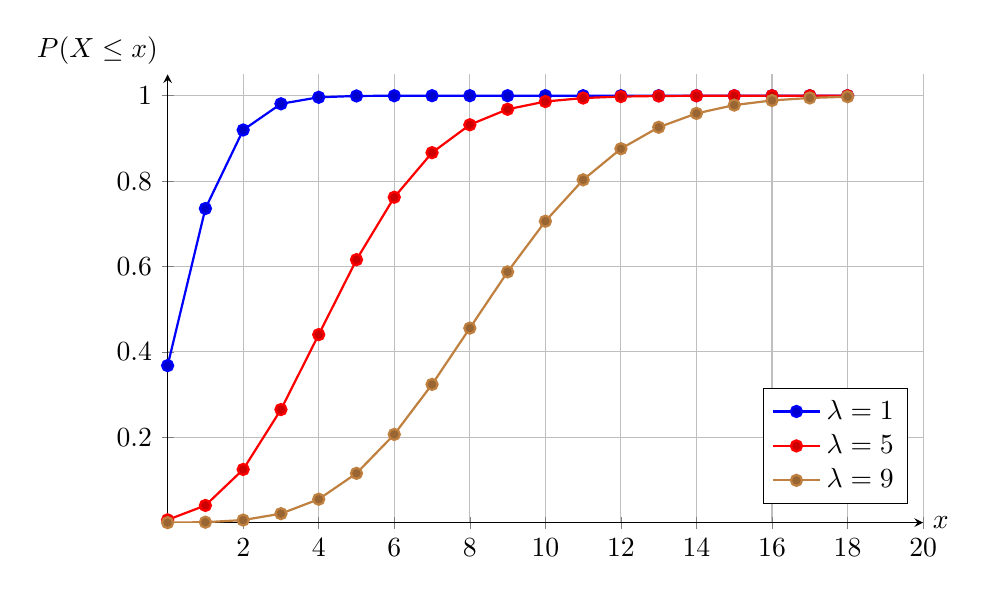
\begin{tikzpicture}
      \begin{axis}[
        axis x line=center,
        axis y line=center,
        xtick={0,2,...,19},
        ytick={0.2,0.4,...,1.0},
        domain = 0:18,
        samples = 19,
        xlabel={$x$},
        ylabel={$P(X\leq x)$},
        xlabel style={right},
        ylabel style={above left},
        ymax=1.05,
        xmax=20,
        grid=major,
        x post scale=1.4,
        legend style={at={(0.98,0.3)},anchor=north east}
        ]
        \addplot+[thick,blue,mark=*] coordinates {
          (0,0.3679) (1,0.7358) (2,0.9197) (3,0.9810) (4,0.9963) 
          (5,0.9994) (6,0.9999) (7,1.0000) (8,1.0000) (9,1.0000)
          (10,1.0000) (11,1.0000) (12,1.0000) (13,1.0000) (14,1.0000)
          (15,1.0000) (16,1.0000) (17,1.0000) (18,1.0000)
        };
        \addlegendentry{$\lambda = 1$}
        \addplot+[thick,red,mark=*] coordinates {
          (0,0.0067) (1,0.0404) (2,0.1247) (3,0.2650) (4,0.4405) 
          (5,0.6160) (6,0.7622) (7,0.8666) (8,0.9319) (9,0.9682)
          (10,0.9863) (11,0.9945) (12,0.9980) (13,0.9993) (14,0.9998)
          (15,0.9999) (16,1.0000) (17,1.0000) (18,1.0000)
        };
        \addlegendentry{$\lambda = 5$}
        \addplot+[thick,brown,mark=*] coordinates {
          (0,0.0001) (1,0.0012) (2,0.0062) (3,0.0212) (4,0.0550) 
          (5,0.1157) (6,0.2068) (7,0.3239) (8,0.4557) (9,0.5874)
          (10,0.7060) (11,0.8030) (12,0.8758) (13,0.9261) (14,0.9585)
          (15,0.9780) (16,0.9889) (17,0.9947) (18,0.9976)
        };
        \addlegendentry{$\lambda = 9$}
      \end{axis}
    \end{tikzpicture}
  \end{center}
\end{frame}

\begin{frame}
  \frametitle{Mean and variance}

  \pause

  The mean $\mathbb{E}(X)$ and variance $\mathbb{V}(X)$ of a Poisson distributed random variable are equivalent \pause
  
  \begin{block}{}
    \begin{equation}
      \mathbb{E}(X) = \mathbb{V}(X) = \sigma^{2}_{X} = \pause \la
    \end{equation}
  \end{block}

    \pause

    {\rd The standard deviation is \pause $\sigma(X) = \sqrt{\mathbb{V}(X)} = \sqrt{\la}$}
  \end{frame}
  
\begin{frame}[fragile]
  \frametitle{Computing Poisson probabilities in Python}
  
% \begin{alertblock}{Matlab}
%   \begin{itemize}[<+->]
%   \item In MATLAB, you compute the PMF $P(X=x)$ using \texttt{poisspdf(x, lambda)}
     
%   \item Similarly, you can find the CDF  $P(X\le x)$ as \texttt{poisscdf(x, lambda)}
    
%   \item Note that $P(X > x)$ is obtained by \\\pause
%     \texttt{poisscdf(x, lambda, `upper')} $\equiv 1 -$  \texttt{poisscdf(x, lambda)}
%  \end{itemize}
% \end{alertblock}

\pause

%\begin{alertblock}{Python}
  \begin{itemize}[<+->]
  \item Load: 
  \pythoninline{from scipy.stats import poisson}
  
  \item Compute the PMF $P(X=x)$ using \pythoninline{poisson.pmf(x, lambda)}

  \item Similarly, you can find the CDF  $P(X\le x)$ as \pythoninline{poisson.cdf(x, lambda)}
    
  \item Note that $P(X > x)$ (survival function) is obtained by \\\pause
  \pythoninline{
    1 -  poisson.cdf(x, lambda)}
    \\ \pause

    or
    \pause

    \pythoninline{
    poisson.sf(x, lambda) # sf = survival function = 1 - cdf}
 \end{itemize}
%\end{alertblock}
\end{frame}




  \section{Examples}
 
\begin{frame}
  \frametitle{Example 1: Amherst Coffee customer arrivals}
  \pause

  Starting at 7 AM, customers arrive Amherst Coffee according to a Poisson process at the rate of 30 customers per
  hour. Find the \pause
  (a) probability that \textbf{exactly 40} customers arrive between 10 and 11 AM; \pause
  (b)  probability that \textbf{no more than 40} customers arrive between 11 AM and 12 PM; \pause
  (c)  \textbf{uncertainty} in the rate parameter.

  \pause

  \begin{exampleblock}{Solution}
    \pause
    The number of customers arriving within an hour $ X\sim \text{Poisson}(\la=30)$.\pause
    \begin{enumerate}[\bf (a)]
    \item  \pause
      The desired probability is given by:\pause
      \begin{equation*}
        P(X = 40) = \fr{30^{40}}{40!}e^{-30} \pause = \pythoninline{poisson.pmf(40,30)} \pause = \boxed{\gr 0.0139}
      \end{equation*}
      \pause
    \item The desired probability is given by: \pause
      \begin{equation*}
        P(X\le 40) =\pause \sum_{k=0}^{40}\fr{30^{k}}{k!}e^{-30}  \pause
                   = \pythoninline{poisson.cdf(40,30)} \pause = \boxed{\gr 0.9677}
      \end{equation*}
    \end{enumerate}
  \end{exampleblock}
\end{frame}

\begin{frame}
  \frametitle{Example 1: Amherst Coffee customer arrivals (cont.)}
  \pause
  \begin{exampleblock}{Solution (cont.)}
    \pause

    \begin{enumerate}[\bf (a)]\setcounter{enumi}{2}
    \item The uncertainty is given by the standard deviation: \pause
      \begin{equation*}
        \sigma_{X} = \sqrt{\la} \pause = \sqrt{30} \pause = \boxed{\gr 5.477}
      \end{equation*}
    \end{enumerate}
  \end{exampleblock}

\end{frame}


\begin{frame}
  \frametitle{Example 2: Aircraft arrivals at airport} \pause Suppose small
    aircraft arrive at a certain airport according to a Poisson process with a
    rate $\la = 8$/hr. \pause

    \begin{enumerate}[(a)]
    \item What is the probability that exactly 6 small aircraft arrive during a 1-hr period?
    \item What is the probability that at least 10 small aircraft arrive during a 1-hr period?
    \item How many aircraft do you expect to arrive during a 90-minute period?  
    \end{enumerate}
    
\end{frame}

\begin{frame}
  \frametitle{Example 2: Aircraft arrivals at airport (cont.)} \pause
    %Given $\la = 8$:

    \begin{enumerate}[(a)]
    \item What is the probability that exactly 6 small aircraft arrive during a 1-hr period?\pause
      
    \begin{exampleblock}{Solution}
      
    \begin{eqnarray*}
        P(X_{1hr} = 6) &=& \fr{\la^x e^{-\la}}{x!} = \pause \fr{8^6e^{-8}}{6!} = \pause
        \pythoninline{poisson.pmf(6,8)} \pause = \boxed{0.1221}
      \end{eqnarray*}
    \end{exampleblock}


      \pause
    \item What is the probability that at least 10 small aircraft arrive during a 1-hr period? \pause
    \begin{exampleblock}{Solution}
      
     % 1-hr period implies $X_{1hr} \sim \text{Poisson}(\la=8)$.\pause

      The desired probability is given by:\pause 
    \begin{eqnarray*}
        P(X_{1hr} > 9) &=& 1 - P(X_{1hr}  \le 9) \\ \pause
                       &=& 1 - \sum_{x =0}^9\fr{\la^x e^{-\la}}{x!} = \pause \pythoninline{1 - poisson.cdf(9,8)} \\ \pause
                       &=& 1 - 0.7166 = \pause \boxed{0.2834}
      \end{eqnarray*}
    \end{exampleblock}
    \end{enumerate}
    
 
\end{frame}

  \begin{frame}
    \frametitle{Manipulating the rate parameter}
    
    \pause

    \begin{itemize}[<+->]

    \item The rate parameter $\la$ is given by the mean number of occurrences per unit time.
      \medskip
      
    \item If we are to find the probability of a certain number of events within a different time interval $T'$, where
      \begin{equation}
        T' = T \times t
      \end{equation}
      \pause
    \item Then, 
      we can find the new rate parameter by  multiplying  $\la$ by the appropriate number of time units $t$, such that
      \begin{equation}
       \la' = \la t
      \end{equation}
      \pause

    \item       And thus:
      \begin{equation}
        P(X_{t} = x) = \fr{(\la t)^{x}}{x!}e^{-(\la t)} = \fr{(\la')^{x}}{x!}e^{-(\la')}
      \end{equation}
    \end{itemize}


  \end{frame}
  
\begin{frame}
  \frametitle{Example 2: Aircraft arrivals at airport (cont.)} \pause
    
    \begin{enumerate}[(a)]\setcounter{enumi}{2}
    \item How many aircraft do you expect to arrive during a 90-minute period? 
      \pause
      \begin{exampleblock}{Solution}
      \pause
      Expected arrivals within 90 minutes = 8/hr $\times$ 1.5 hrs = \pause 12.
      \end{exampleblock}
    \end{enumerate}
    
 
\end{frame}


 \begin{frame}
  \frametitle{Example 3: Amherst Coffee customer arrivals (revisited)}
  \pause

  Starting at 7 AM, customers arrive Amherst Coffee according to a Poisson process at the rate of 30 customers per
  hour. Now find the probability more than 65 customers arrive between 10 and 12 PM. 

  \pause

  \begin{exampleblock}{Solution}
    \pause

    The probability is now desired for an interval twice as long. \pause So we compute a new rate parameter for 2-hr interval: \pause

    \begin{equation*}
      \la^{*} = \pause 30 \times 2 \pause = 60 \text{ (per 2 hrs)}
    \end{equation*}
    \pause
      The desired probability is thus given by:\pause
      \begin{eqnarray*}
        P(X_{2 hr} > 65) &=& \pause 1- P(X_{2 hr}\le 65) \pause = 
        \pythoninline{1 - poisson.cdf(65,60)} \\\pause 
        &\equiv& 
        \pythoninline{poisson.sf(65,60)} \pause = \boxed{0.2355}
      \end{eqnarray*}

    \end{exampleblock}
  \end{frame}


  
  \begin{frame}
    \frametitle{Example 4: Text messages}
    \pause

    A student receives text messages starting at 10 AM at the rate of 10 texts per hour according to a Poisson process. Find the probability that they will recieve exactly 18 texts by noon and 70 texts by 5 PM.

    \pause

    \begin{exampleblock}{Solution}
      \pause

      \begin{itemize}[<+->]\item 
        The student receives 18 texts in the first 2 hrs and then $70-18=52$ texts in the next 5 hrs (5:00 PM).

      \item The events $X_{12}=18$ and $X_{5}=52$ are independent within the specified time intervals.

    \end{itemize}

    \pause

    Thus:
    \begin{eqnarray*}
      P(X_{12}=18 \cap X_{5}=52) &=& \pause P(X_{12}=18) \times P(X_{5}=52) \\\pause
                                &=& \fr{(10(2))^{18}}{18!}e^{-10(2)} \times \fr{(10(5))^{52}}{52!}e^{-10(5)} \\\pause
                                &=& \pythoninline{poisson.pmf(18,20) * poisson.pmf(52,50)} \\\pause
                                &=& \boxed{\gr 0.0045}
    \end{eqnarray*}

    \end{exampleblock}
  \end{frame}
  
\section{Outlook}

 \begin{frame}
  \frametitle{Poisson distribution as limit of binomial distribution} \pause

      For a binomially distributed r.v.\ $X$ with $n$ trials, \pause
      as $n\to \infty$ and $p\to 0$, then \pause
      \begin{equation}
        \label{eq:43}
        X\sim \text{Bin}(n,p) \to X \sim \text{Poisson}(\la)
      \end{equation} \pause
      where $\la = np$. 

      \pause

     \begin{tikzpicture}[
      declare function={binom(\k,\n,\p)=\n!/(\k!*(\n-\k)!)*\p^\k*(1-\p)^(\n-\k);}
      ]
      \begin{axis}[
        height=9cm,
        width=10cm,
        samples at={0,...,100},
        xlabel=$x$,
        ylabel=$P(x)$,
        xlabel style={right},
        ylabel style={above left},
        xtick={0,20,...,100},
        ytick={0.05,0.1,0.15},
        axis x line=center,
        axis y line=center,
        xmax = 105,
        ymax =.15,
        y post scale = .7,
        x post scale=1.2,
        legend style={at={(1, 1)},anchor=north east},
        yticklabel style={
          /pgf/number format/fixed,
          /pgf/number format/fixed zerofill,
          /pgf/number format/precision=2
        }
        ]
        \only<7->{\addplot+[ycomb,opacity=.5] {binom(x,100,0.2)}; \addlegendentry{Bin$(100,0.20)$}}
        \only<8->{\addplot+[ycomb,opacity=.5] {poiss(20))};}
        \only<9->{\addlegendentry{Poisson$(20)$};}
        \only<10->{\addplot+[very thick,samples=100,opacity=.5,no markers] {gauss(20,4)};}
        \only<11->{\addlegendentry{$\mathcal{N}(\mu =20, \sigma=4)$};}     
        \only<12->{\addplot+[ycomb,opacity=.5] {binom(x,100,0.4)}; \addlegendentry{Bin$(100,0.40)$}}
        \only<13->{\addplot+[ycomb,opacity=.5] {poiss(40))};}
        \only<14->{\addlegendentry{Poisson$(40)$};}
        \only<15->{\addplot+[very thick,samples=100,opacity=.5,no markers] {gauss(40,4.899)};}
        \only<16->{\addlegendentry{$\mathcal{N}(\mu =40, \sigma=4.9)$};}
      \end{axis}
    \end{tikzpicture}
\end{frame}



\begin{frame}
  \frametitle{Recap}
  \begin{itemize}[<+->]
  \item The Poisson distribution is used to model the probability that a number of independent events occur within a fixed time interval (or within a finite space)

  \item Such events are described as \textbf{Poisson processes}

  \item The \textbf{PMF} of a Poisson random variable with rate parameter $\la$ is given by:
    \begin{equation}
      P(X=x) = \fr{\la^{x}}{x!} e^{-\la}
    \end{equation}
    where $x \ge 0$

  \item The \textbf{mean} and \textbf{variance} of a Poisson random variable are equal:
    \begin{equation}
      \mathbb{E}(X) = \mathbb{V}(X) = \la
    \end{equation}

  \item Recall that the \textbf{standard deviation} is simply the square root of the variance:
    \begin{equation}
      \sigma(X) = \sqrt{\la}
    \end{equation}
  \end{itemize}
  \pause
  
  \begin{block}{Reading}
    \begin{itemize}
    \item Open Intro Statistics Section 4.5 
    \end{itemize}
  \end{block}
\end{frame}




%\backupbegin
% \section{Appendix}



% \begin{frame}
%   \frametitle{Skewness}\pause
%   The skewness or symmetry of a distribution is measured by the third central moment: \pause

%   In the discrete case: \pause
%     \begin{equation}
%       \label{eq:var}
%       \mathbb{E}(X - \mu_X)^3 = \sum_i(x_i - \mu_X)^3p_X(x_i)
%     \end{equation}
%     \pause

%     In the continuous case:\pause
%     \begin{equation}
%       \label{eq:6}
%       \mathbb{E}(X - \mu_X)^3 = \int_{-\infty}^{\infty}(x - \mu_X)^3 f_X(x)dx
%     \end{equation}

%     \pause

%     For convenience, the skewness coefficient is also used (unitless):\pause

%     \begin{equation}
%       \label{eq:7}
%       \theta = \fr{\mathbb{E}(X - \mu_X)^3}{\sigma^3}
%     \end{equation}
    
% \end{frame}

% \begin{frame}
%   \frametitle{Skewness (cont.)}
%   \pause

%   \begin{itemize}[<+->]
%   \item Positive skewness is characterized by a long right tail (right-skewed)
%   \item Negative skewness is characterized by a long left tail (left-skewed)
%   \end{itemize}

%   \pause

%   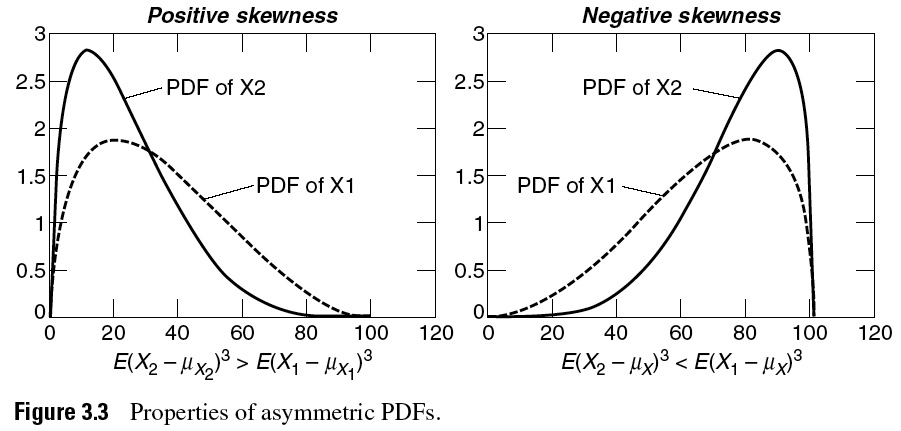
\includegraphics[width=\textwidth,trim={0 2cm 0 0},clip]{03_03}
  
% \end{frame}
% \begin{frame}
%   \frametitle{Kurtosis} \pause

%   This is the measure of peakedness in a distribution. \pause It is the fourth central moment: \pause

  
%   In the discrete case: \pause
%     \begin{equation}
%       \label{eq:8}
%       \mathbb{E}(X - \mu_X)^4 = \sum_i(x_i - \mu_X)^4p_X(x_i)
%     \end{equation}
%     \pause

%     In the continuous case:\pause
%     \begin{equation}
%       \label{eq:6}
%       \mathbb{E}(X - \mu_X)^4 = \int_{-\infty}^{\infty}(x - \mu_X)^4 f_X(x)dx
%     \end{equation}


% \end{frame}

% \begin{frame}
%   \frametitle{Skewness vs. kurtosis}
%   \pause

%   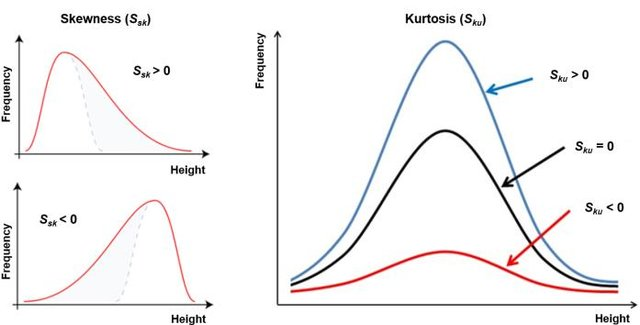
\includegraphics[width=\textwidth]{skewness-kurtosis}

%   {\tiny Source: Bonyar, A (2015) ``Application of localization factor for the detection of tin oxidation with AFM'' DOI: 10.1109/SIITME.2015.7342289}
% \end{frame}

% \begin{frame}
%   \frametitle{Generalized expectation}
%   The mathematical expectation can be defined for a function $g$ of random variable $X$:
  
%      \begin{align}
%       E[g(X)] &= \sum_i g(x_i) p_X(x_i) \quad \text{\og discrete case}\\ \pause
%       E[g(X)] &= \int_{-\infty}^{\infty}g(x)f_X(x)dx \quad \text{\og continuous case}
%     \end{align}

%   \end{frame}
  

%\backupend

%\begin{frame}[allowframebreaks]
%   \frametitle{References}
%   \AtNextBibliography{\scriptsize}
%   \setbeamertemplate{bibliography item}[text]
%   \printbibliography[heading=none]
  
% \end{frame}

%\printbibliography
\end{document}
%%% Local Variables:
%%% mode: latex
%%% TeX-master: t
%%% End:
